\documentclass{article}
\usepackage{graphicx}
\usepackage{fullpage,latexsym,picinpar,amsmath,amsfonts}
\usepackage{amssymb}
\usepackage[section]{placeins}

           

%%%%%%%%%%%%%%%%%%%%%%%%%%%%%%%%%%%%%%%%%%%%%%%%%%%%%%%%%%%%%%%%%%%%%%%%%%%%%%%%%%%
%%%%%%%%%%%  LETTERS 
%%%%%%%%%%%%%%%%%%%%%%%%%%%%%%%%%%%%%%%%%%%%%%%%%%%%%%%%%%%%%%%%%%%%%%%%%%%%%%%%%%%

\newcommand{\barx}{{\bar x}}
\newcommand{\bary}{{\bar y}}
\newcommand{\barz}{{\bar z}}
\newcommand{\bart}{{\bar t}}

\newcommand{\bfP}{{\bf{P}}}

%%%%%%%%%%%%%%%%%%%%%%%%%%%%%%%%%%%%%%%%%%%%%%%%%%%%%%%%%%%%%%%%%%%%%%%%%%%%%%%%%%%
%%%%%%%%%%%%%%%%%%%%%%%%%%%%%%%%%%%%%%%%%%%%%%%%%%%%%%%%%%%%%%%%%%%%%%%%%%%%%%%%%%%
                                                                                
\newcommand{\parend}[1]{{\left( #1  \right) }}
\newcommand{\spparend}[1]{{\left(\, #1  \,\right) }}
\newcommand{\angled}[1]{{\left\langle #1  \right\rangle }}
\newcommand{\brackd}[1]{{\left[ #1  \right] }}
\newcommand{\spbrackd}[1]{{\left[\, #1  \,\right] }}
\newcommand{\braced}[1]{{\left\{ #1  \right\} }}
\newcommand{\leftbraced}[1]{{\left\{ #1  \right. }}
\newcommand{\floor}[1]{{\left\lfloor #1\right\rfloor}}
\newcommand{\ceiling}[1]{{\left\lceil #1\right\rceil}}
\newcommand{\barred}[1]{{\left|#1\right|}}
\newcommand{\doublebarred}[1]{{\left|\left|#1\right|\right|}}
\newcommand{\spaced}[1]{{\, #1\, }}
\newcommand{\suchthat}{{\spaced{|}}}
\newcommand{\numof}{{\sharp}}
\newcommand{\assign}{{\,\leftarrow\,}}
\newcommand{\myaccept}{{\mbox{\tiny accept}}}
\newcommand{\myreject}{{\mbox{\tiny reject}}}
\newcommand{\blanksymbol}{{\sqcup}}
                                                                                                                         
\newcommand{\veps}{{\varepsilon}}
\newcommand{\Sigmastar}{{\Sigma^\ast}}
                           
\newcommand{\half}{\mbox{$\frac{1}{2}$}}    
\newcommand{\threehalfs}{\mbox{$\frac{3}{2}$}}   
\newcommand{\domino}[2]{\left[\frac{#1}{#2}\right]}  

%%%%%%%%%%%% complexity classes

\newcommand{\PP}{\mathbb{P}}
\newcommand{\NP}{\mathbb{NP}}
\newcommand{\PSPACE}{\mathbb{PSPACE}}
\newcommand{\coNP}{\textrm{co}\mathbb{NP}}
\newcommand{\DLOG}{\mathbb{L}}
\newcommand{\NLOG}{\mathbb{NL}}
\newcommand{\NL}{\mathbb{NL}}

%%%%%%%%%%% decision problems

\newcommand{\PCP}{\sc{PCP}}
\newcommand{\Path}{\sc{Path}}
\newcommand{\GenGeo}{\sc{Generalized Geography}}

\newcommand{\malytm}{{\mbox{\tiny TM}}}
\newcommand{\malycfg}{{\mbox{\tiny CFG}}}
\newcommand{\Atm}{\mbox{\rm A}_\malytm}
\newcommand{\complAtm}{{\overline{\mbox{\rm A}}}_\malytm}
\newcommand{\AllCFG}{{\mbox{\sc All}}_\malycfg}
\newcommand{\complAllCFG}{{\overline{\mbox{\sc All}}}_\malycfg}
\newcommand{\complL}{{\bar L}}
\newcommand{\TQBF}{\mbox{\sc TQBF}}
\newcommand{\SAT}{\mbox{\sc SAT}}

%%%%%%%%%%%%%%%%%%%%%%%%%%%%%%%%%%%%%%%%%%%%%%%%%%%%%%%%%%%%%%%%%%%%%%%%%%%%%%%%%%%
%%%%%%%%%%%%%%% for homeworks
%%%%%%%%%%%%%%%%%%%%%%%%%%%%%%%%%%%%%%%%%%%%%%%%%%%%%%%%%%%%%%%%%%%%%%%%%%%%%%%%%%%

\newcommand{\student}[2]{%
{\noindent\Large{ \emph{#1} SID {#2} } \hfill} \vskip 0.1in}

\newcommand{\assignment}[1]{\medskip\centerline{\large\bf CS 111 ASSIGNMENT {#1}}}

\newcommand{\duedate}[1]{{\centerline{due {#1}\medskip}}}     

\newcounter{problemnumber}                                                                                 

\newenvironment{problem}{{\vskip 0.1in \noindent
              \bf Problem~\addtocounter{problemnumber}{1}\arabic{problemnumber}:}}{}

\newcounter{solutionnumber}

\newenvironment{solution}{{\vskip 0.1in \noindent
             \bf Solution~\addtocounter{solutionnumber}{1}\arabic{solutionnumber}:}}
				{\ \newline\smallskip\lineacross\smallskip}

\newcommand{\lineacross}{\noindent\mbox{}\hrulefill\mbox{}}

\newcommand{\decproblem}[3]{%
\medskip
\noindent
\begin{list}{\hfill}{\setlength{\labelsep}{0in}
                       \setlength{\topsep}{0in}
                       \setlength{\partopsep}{0in}
                       \setlength{\leftmargin}{0in}
                       \setlength{\listparindent}{0in}
                       \setlength{\labelwidth}{0.5in}
                       \setlength{\itemindent}{0in}
                       \setlength{\itemsep}{0in}
                     }
\item{{{\sc{#1}}:}}
                \begin{list}{\hfill}{\setlength{\labelsep}{0.1in}
                       \setlength{\topsep}{0in}
                       \setlength{\partopsep}{0in}
                       \setlength{\leftmargin}{0.5in}
                       \setlength{\labelwidth}{0.5in}
                       \setlength{\listparindent}{0in}
                       \setlength{\itemindent}{0in}
                       \setlength{\itemsep}{0in}
                       }
                \item{{\em Instance:\ }}{#2}
                \item{{\em Query:\ }}{#3}
                \end{list}
\end{list}
\medskip
}

%%%%%%%%%%%%%%%%%%%%%%%%%%%%%%%%%%%%%%%%%%%%%%%%%%%%%%%%%%%%%%%%%%%%%%%%%%%%%%%%%%%
%%%%%%%%%%%%% for quizzes
%%%%%%%%%%%%%%%%%%%%%%%%%%%%%%%%%%%%%%%%%%%%%%%%%%%%%%%%%%%%%%%%%%%%%%%%%%%%%%%%%%%

\newcommand{\quizheader}{ {\large NAME: \hskip 3in SID:\hfill}
                                \newline\lineacross \medskip }


%%%%%%%%%%%%%%%%%%%%%%%%%%%%%%%%%%%%%%%%%%%%%%%%%%%%%%%%%%%%%%%%%%%%%%%%%%%%%%%%%%%
%%%%%%%%%%%%% for final
%%%%%%%%%%%%%%%%%%%%%%%%%%%%%%%%%%%%%%%%%%%%%%%%%%%%%%%%%%%%%%%%%%%%%%%%%%%%%%%%%%%

\newcommand{\namespace}{\noindent{\Large NAME: \hfill SID:\hskip 1.5in\ }\\\medskip\noindent\mbox{}\hrulefill\mbox{}}



\begin{document}

\centerline{\large \bf CS/MATH111 ASSIGNMENT 2}
\centerline{Itzel Gonzalez SID: 861304050 and Jiunn Siow SID:861196669}
\centerline{April 2019}

\vskip 0.1in
%\noindent{\bf Individual assignment:} Problems 1 and 2.

%\noindent{\bf Group assignment:} Problems 1,2 and 3.

\vskip 0.2in

%%%%%%%%%%%%PROBLEM1%%%%%%%%%%%%%%%%
\begin{problem}
Let $n = p_1 p_2 ... p_k$, where $p_1, p_2, ..., p_k$ are different primes. Prove that $n$ has exactly $2^k$ different divisors. 
For example, if $n = 105$, then n = $3 \cdot 5 \cdot 7$, so $k = 3$, and thus $n$ has $2^3 = 8$ divisors. These divisors are: $1, 3, 5, 7, 15, 21, 35, 105$.
Hint. You can reduce the problem to counting other objects that we already know how to count. Alternatively, this can be proved by induction on $k$.
\end{problem}
\begin{solution}
\text{We will be using Induction to prove this problem}
\\
\textbf{Base case:}
\\
\text{Assume that k = 1.}
\text{As a result, we should get 2 divisors if we have one  prime $p_1$.}
\\
\text{Assume that n is any prime number. As a result we know that the two divisors are 1 and n itself}
\\
\text{Therefore, the base case holds}
\\
\textbf{Inductive Step:}
\\
\text{We want to prove that for $n = p_1 p_2 ... p_k$,that there are different prime numbers that there} 
\text{are $2^k$ different divisors}
\\
\text{Assumption: We know that for $n = p_1 p_2 ... p_{k-1}$ that there k-1 different primes and there are $2^{k-1}$ different divisors.}
\\
\begin{alignat*}{2}
    & n_1 = p_1 p_2 ... p_{k-1}
    && \hspace{20} \text{Following our assumption with a certain number $n_1$}
    \\
    & n_2 = n_1 \cdot p_k 
    && \hspace{20} \text{Multiply every prime number in $n_1$ by $p_k$ to get a new divisor for each old divisor}
    \\
    & d_1 \cdot p^{k} = d_2 
    && \hspace{20} \text{$d_1$ is the set of all divisors from $n_1$.$d_2$ is the new set of divisors $d_1$ multiplied by $p_k$}
    \\
    & ...d_{1_{k-1}} \cdot p^{k} = ...d_{2_{k-1}}
\end{alignat*}
\text{We need to add all the old and new divisors together. We know for both $n_1$ and $n_2$, that there are $2^{k-1}$ divisors}
\begin{alignat*}{2}
    & 2^{k} = d_1 + d_2
    && \hspace{20} \text{Following from before }
    \\
    & 2^k = 2^{k-1} + 2^{k-1}
    && \hspace{20} \text{Counting current primes and new primes}
    \\
    & 2^k = \frac{1}{2} \cdot 2^{k} + \frac{1}{2} \cdot 2^{k-1}
\end{alignat*}
\text{Therefore, by induction we know that for $n = p_1 p_2 ... p_k$ that there are $2^{k}$ divisors.}
\\
\text{We accounted for all the divisors that either contained $p_k$ or did not contain $p_k$.}
\\
\text{$d_1$ contained all the divisors that did not contain $p_k$ and $d_2$ accounted for divisors that contained $p_k$}
\end {solution}
%%%%%%%%%%%%PROBLEM2%%%%%%%%%%%%%%%%
\begin{problem}
Alice's RSA public key is $P = (e,n) = (13,77)$.
Bob sends Alice the message by encoding it as follows.
First he assigns numbers to characters:
A is 2, B is 3, ..., Z is 27, and blank is 28. Then he
uses RSA to encode each number separately. 

Bob's encoded message is:

\begin{verbatim}
     10       7      58      30      23      62 
      7      64      62      23      62      61 
      7      41      62      21       7      49 
     75       7      69      53      58      37 
     37      41      10      64      50       7 
     10      64      21      62      61      35 
     62      61      62       7      52      10 
     21      58       7      49      75       7 
     62      26      22      53      30      21 
     10      37      64
 \end{verbatim}

Decode Bob's message.
Notice that you don't have Bob's secrete key, so you
need to ``break" RSA to decrypt his message.

\smallskip
For the solution, you need to provide the following:
%
\begin{itemize}
%
\item Describe step by step how you arrived at the solution.
	In particular, explain how you determined $p$, $q$, $\phi(n)$, and $d$.
%
\item Show the calculation that determines the first letter in the message from the first number in ciphertext.
%
\item Give Bob's message in plaintext. The message is a quote. Who said it?
%
\item If you wrote a program, attach your code to the hard copy.
	If you solved it by hand (not recommended), attach your scratch paper with calculations
	for at least 5 first letters.
%
\end{itemize}

Suggestion: this can be solved by hand, but it will probably
be faster to write a short program.
\end{problem}

\begin{solution}
\begin{itemize}
%
\item Describe steps of solution:\\
	We find p and q from n, we are given n = 77.\\ 
	The only prime factors of 77 are 7 and 11.\\
	So, p = 7 and q = 11.\\
	
	Next, we find totient function $\phi(n)$.\\ $\phi(77) = (p-1)(q-1) = 6*10 = 60$\\
	
	Next, we solve for d using formula: $d = e^{-1}mod(\phi(n))$\\
	Plugging in $e = 13$ and $\phi(n) = 60$: $d = 13^{-1}mod(60)$\\
	 Since 60 is not prime, we cannot use Fermat's Little Theorem\\ 
	\\
	But we can use Euclid's Algorithm: $gcd(60, 13)$\\
	$60 = 13(4) + 8 \rightarrow 8 = 60 - 13(4)$\\
	$13 = 8(1) + 5 \rightarrow 5 = 13 - 8$\\
	$8 = 5(1) + 3 \rightarrow 3 = 8 - 5$\\
	$5 = 3(1) + 2 \rightarrow 2 = 5 - 3$\\
	$3 = 2(1) + 1 \rightarrow 1 = 3 - 2$\\
	
	$1 = 3 - [5 - 3] \rightarrow 1 = 2(3) - 5$\\
	$1 = 2[8 - 5] - 5 \rightarrow 1 = 2(8) - 3(5)$\\
	$1 = 2[8 - 5] - 5 \rightarrow 1 = 5(8) - 3(13)$\\
	$1 = 5[60 - 4(13)] - 3(13) \rightarrow 1 = 5(60) - 20(13) - 3(13)$\\
	$1 = 5(60)-23(13)$\\
	$d = -23 mod(60) \rightarrow d = 37$\\
	
	Next, we decrypt message using formula: $M = C^d mod(n)$\\
	Our formula is: $M = C^{37} mod(77)$\\
%
\item We can decrypt the letter for the first number in the ciphertext using C = 10.\\
%
    $M = C^{37} mod(77) \rightarrow M = 10^{37} mod(77)$\\
    $M = (10^2)^{18}*10mod(77)$\\
    $10^{2} mod(77) = 23$\\
    $10^{4} mod(77) = (10^{2})^{2}mod(77) = (23)^2 mod(77) = 67$\\
    $10^{8} mod(77) = (10^{4})^{2}mod(77) = (67)^2 mod(77) = 23$\\
    $10^{16} mod(77) = (10^{8})^{2}mod(77) = (23)^2 mod(77) = 67$\\
    $10^{32} mod(77) = (10^{16})^{2}mod(77) = (67)^2 mod(77) = 23$\\
    $10^{37} mod(77) = (10^{32}*10^{4}*10)mod(77) = (23*67*10) mod(77) = 10$\\
    $M = 10$
\item Give Bob's message in plaintext. The message is a quote. Who said it?\\
%
``I HAVE NEVER LET MY SCHOOLING INTERFERE WITH MY EDUCATION" by Mark Twain
%
	\begin{figure}[h]
	\centerline{Code for RSA Decryption:}
    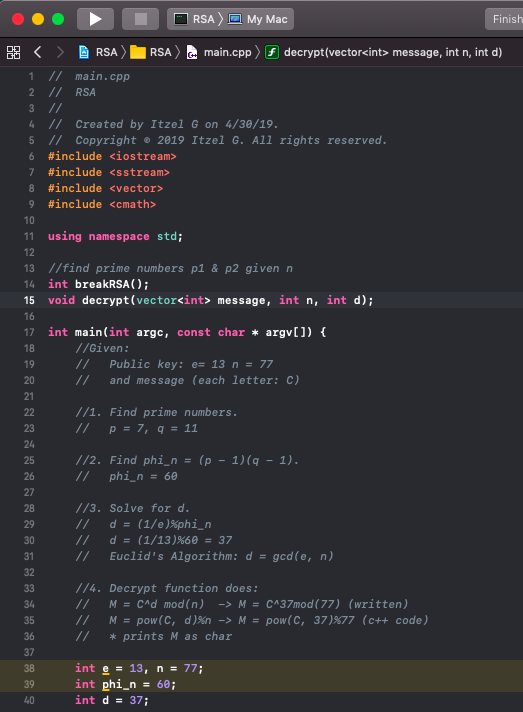
\includegraphics[width=116mm,,scale=1.5]{1.png}
    \end{figure}
    \begin{figure}
    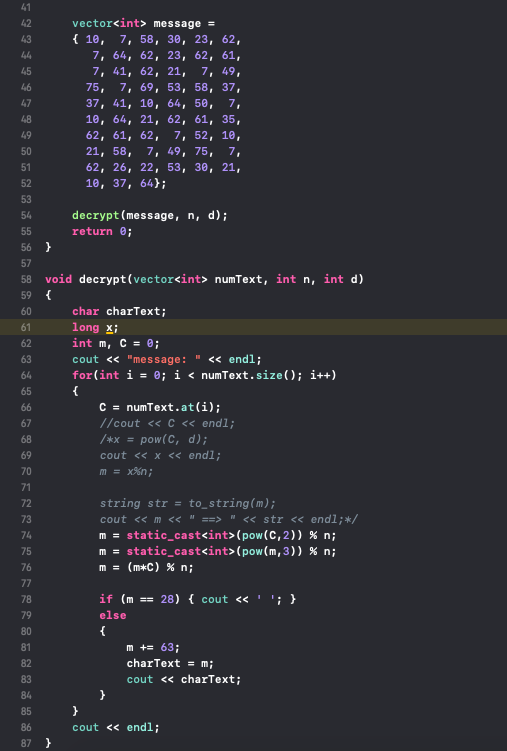
\includegraphics[width=150mm,,scale=1.5]{2.png}
    \end{figure}
    \begin{figure}
    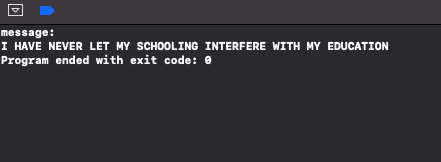
\includegraphics[width=150mm,,scale=1.5]{3.png}
    \end{figure}
    \end{itemize}
\end {solution}
\newpage 
%%%%%%%%%%PROBLEM3%%%%%%%%%%%%%%%%%%
\begin{problem}
\\

(a) Compute $13^{-1}\pmod{19}$ by enumerating multiples of the number and the modulus.
Show your work.
\\
\text{Referring to the slides in number theory. We want to find an integer a and b that satisfies } $13^{-1}\pmod{19}$
\\
\begin{alignat*}{2}
    & a = 13^{-1}\pmod{19}
    && \hspace{20} \text{Multiply both sides by 13}
    \\
    & 13 \cdot a = 1\pmod{19} 
    && \hspace{20} \text{turn into multiple form}
    \\
    & 13\cdot a = 19\cdot b + 1
\end{alignat*}
\text{On the LHS, we have multiples 13,26,29. On the RHS, we have multiples 20,39,58.}
\\
\text{Since $39 = 19 \cdot 2 + 1$, we have $a=3$ and $b =2$.So as a result we have $13^{-1}= 3\pmod{19}$}.
\\
\text{Finally, substituting what we just found $13^{-1}\pmod{19}= 3\pmod{19}$}
\\
\smallskip\noindent

(b) Compute $13^{-1}\pmod{19}$ using Fermat's theorem. Show your work.
\\
\text{Referring to the slides in number theory. We want to find use Fermat's little Theorem}
\\
\begin{alignat*}{2}
    & a^{p-1} = 1\pmod{p}
    && \hspace{20} \text{If p is a prime number, and a is not divisible by p(FLT)}
    \\
    & 13^{19-1} = 1\pmod{19} 
    && \hspace{20} \text{ Multiplying, we get this}
    \\
    & 13^{18} = 1\pmod{19}
\end{alignat*}
\text{Next we apply FLT to our equation. We will use what we just found above}
\\
\begin{alignat*}{2}
    & 13^{18} \cdot 13^{-1} = 1\pmod{19}
    && \hspace{20} \text{If p is a prime number, and a is not divisible by p(FLT)}
    \\
    & 13^{17} = 1\pmod{19} 
    && \hspace{20} \text{ Multiplying, we get this}
\end{alignat*}
\text{Listing out exponential and their remainders. This will help us get the final answer }
\\
\begin{alignat*}{2}
    & 13^{2} \pmod{19} = 17
    \\
    & 13^{4} \pmod{19} = 4
    \\
    & 13^{8} \pmod{19} = 16
    \\
    & 13^{16} \pmod{19} = 9
\end{alignat*}
\text{Applying what we just found}
\begin{alignat*}{2}
    & 13^{17} \pmod{19} = 13^{16} \cdot 13^{1} \pmod{19}
    && \hspace{20} \text{We know that $13^{16} \pmod{19} = 9$}
    \\
    & 13^{16} \cdot 13^{1} \pmod{19} = 9 \pmod{19} \cdot 13 \pmod{19}
    \\
    & 9\pmod{19} \cdot 13 \pmod{19} = 142 \pmod{19}
    \\
    & 117\pmod{19} = 3
\end{alignat*}
\text{This matches our final answer in (a). Therefore $13^{-1}\pmod{19}= 3\pmod{19}$ }\\

\smallskip\noindent
(c) Compute $13^{-40}\pmod{19}$ using Fermat's theorem. Show your work.
For this equation 
    \begin{alignat*}{2}
        & a^{p-1} = 1\pmod{p}
        && \hspace{20} \text{If p is a prime number, and a is not divisible by p(FLT)}
        \\
        & 13^{19-1} = 1\pmod{19} 
        && \hspace{20} \text{ Multiplying, we get this}
        \\
        & 13^{18} = 1\pmod{19}
    \end{alignat*}
    \text{Next we apply FLT to our equation. We will use what we just found above}
    \\
     \begin{alignat*}{2}
    & 13^{18}*13^{-40}\pmod{19} \equiv 13^{-22}\pmod{19}
    \\
    & 13^{18}*13^{-22}\pmod{19}\equiv 13^{-4}\pmod{19}
    \\
    & 13^{18}*13^{-4}\pmod{19}\equiv 13^{14}\pmod{19}
    \\
    \end{alignat*}
    
    Listing out exponential and their remainders, will help us find answer for $13^{14}\pmod{19}$
\begin{alignat*}{2}
    &13^{2} \pmod{19} = 17
    \\
    &13^{4} \pmod{19} = 4 
    \\
    & 13^{8} \pmod{19} = 16
\end{alignat*}
\begin{alignat*}{2}
        &13^{14}\pmod{19} = (13^{8}*13^{4}*13^{2})\pmod{19}
        \\
        &13^{14} = (16*4*17)\pmod{19}
        \\
        & = (1088)\pmod{19}
        \\
        & = 5 
        &&\hspace{2} \text{Final answer}
    \end{alignat*}
\smallskip\noindent

(d) Find a number $x\in\braced{1,2,...,36}$
	such that $8x \equiv 3 \pmod{37}$. Show your work.
	(You need to follow the method covered in class; brute-force checking
	all values of $x$ will not be accepted.)
\end{problem}

\begin{alignat*}{2}
    & 8x \equiv 3\pmod{37}
    && \hspace{20} \text{Multiply both sides by the inverse of 8}
    \\
    & 8^{-1} \cdot 8x \equiv 3\pmod{37} \cdot 8^{-1}
    \\
    &  x \equiv 3\pmod{37} \cdot 8^{-1}
\end{alignat*}
\text{Solving for $8^{-1}\pmod{37}$}
\begin{alignat*}{2}
    & a = 8^{-1}\pmod{37}
    && \hspace{20} \text{Multiply both sides by 8}
    \\
    & 8 \cdot a = 37 \cdot b +1 
    && \hspace{20} \text{turn into multiple form}
    \\
\end{alignat*}
\text{Listing out multiples on the RHS: 37,75,112. We know that 112 is divisible by 8.}
\\
\text{Therefore we have $a=14$ and $b =3$.At the end we know that $8^{-1}\pmod{37}= 14\pmod{37}$ }
\\
\text{Plugging it in and solving, we get}
\begin{alignat*}{2}
    & x = 3 \cdot 14 \pmod{37}
    && \hspace{20} \text{Multiply}
    \\
    & x = 42 \pmod{37}
    && \hspace{20} \text{Get remainder}
    \\
    & x = 5
    &&\hspace{20} \text{Final answer}
\end{alignat*}

%%%%%%%%%%%%%%%%%%%%%%%%%%%%

\vskip 0.1in
\paragraph{Submission.}
To submit the homework, you need to upload the pdf file into gradescope
by Friday, May 4 (noon).

%%%%%%%%%%%%%%%%%%%%%%%%%%%%%%%%%%%%%%%%%%%%%%%%%%%%%%%%%%%%%%%%%%%%%


\end{document}

